\chapter{Tổng quan về bài toán và cơ sở lý thuyết}
\label{ch:ly-thuyet}

\section{Tổng quan về mô hình ngôn ngữ lớn}

Mô hình ngôn ngữ lớn là các mô hình học sâu được huấn luyện trên khối lượng văn bản lớn, có khả năng hoàn thành, tóm tắt, trả lời và sinh nội dung theo ngữ cảnh. Trong ứng dụng thực tế, LLM thường không đứng một mình mà được bọc bởi lớp ứng dụng: giao diện người dùng, kho tri thức, công cụ gọi ngoài, và chính sách an toàn. Khả năng ``làm theo chỉ dẫn bằng ngôn ngữ tự nhiên'' cũng chính là điểm yếu khi chỉ dẫn độc hại được đưa vào cùng kênh dữ liệu với chỉ dẫn hệ thống.

\section{Kiến trúc hệ thống ứng dụng mô hình ngôn ngữ lớn}

Một kiến trúc phổ biến là RAG: (1)~người dùng gửi câu hỏi; (2)~hệ thống truy hồi đoạn tài liệu liên quan; (3)~mô hình sinh câu trả lời dựa trên ngữ cảnh truy hồi và chỉ dẫn hệ thống. Các thành phần bổ sung có thể gồm bộ lọc đầu vào/đầu ra, nhật ký kiểm toán, và lớp ủy quyền nguồn tài liệu. Trong đề tài, đường đánh giá chính dùng Mock LLM Provider (hành vi tất định, không gọi mạng) để ưu tiên tính tái lập và kiểm thử; cơ chế truy hồi là \emph{lai} (hybrid), kết hợp BM25 (SQLite FTS5) với embedding vector, thay vì chỉ dựa trên một vector store thuần tuý.

\section{Các rủi ro an toàn trong hệ thống LLM}

\subsection{Prompt injection}

Prompt injection là kỹ thuật khiến mô hình ưu tiên chỉ dẫn của kẻ tấn công hơn chỉ dẫn hệ thống, ví dụ yêu cầu ``bỏ qua mọi chính sách trước đó''~\cite{perez2022ignore}. Dạng gián tiếp (indirect prompt injection) xảy ra khi chỉ dẫn độc hại nằm trong tài liệu/email được nạp vào ngữ cảnh RAG~\cite{owasp_llm_top10,greshake2023indirect}.

\subsection{Rò rỉ dữ liệu và thông tin nhạy cảm}

Hệ thống có thể phát tán PII, bí mật giả định, hoặc nội dung nội bộ nếu đầu ra không được kiểm soát, hoặc nếu gói bàn giao chứa file log/dữ liệu thô (JSONL, \texttt{result.json}, cơ sở dữ liệu tạm).

\subsection{Đầu ra không an toàn}

Ngoài rò rỉ, đầu ra có thể chứa hướng dẫn lạm dụng, nội dung độc hại, hoặc khẳng định sai sự thật. Lớp output guard và chính sách từ chối an toàn nhằm giảm rủi ro này ở mức rule-based lab.

\subsection{Sai lệch hoặc nội dung không đáng tin cậy}

Mô hình có thể ``ảo giác'' hoặc bị thao túng bởi ngữ cảnh độc. Cơ chế provenance/trust và giới hạn nguồn tài liệu phía máy chủ giảm phụ thuộc mù quáng vào nội dung truy hồi.

\subsection{Rủi ro từ dữ liệu, truy vấn Text-to-SQL và tác tử tích hợp công cụ (Multi-Tool Agent)}

Khi LLM được kết nối với cơ sở dữ liệu quan hệ (Text-to-SQL) hoặc được cấp các công cụ thực thi (gửi email, tạo phiếu hỗ trợ, tra cứu đơn hàng), bề mặt tấn công mở rộng thêm hai hình thái nguy hiểm: (i)~\textbf{Prompt-to-SQL Injection (P2SQL)} trực tiếp, trong đó kẻ tấn công lừa mô hình sinh câu lệnh SQL vượt quyền đọc các bảng/cột nhạy cảm (\texttt{UNION SELECT}, truy vấn lồng nhau, CTE đệ quy gây cạn kiệt tài nguyên hoặc câu lệnh ghép \texttt{DROP/DELETE}); và (ii)~\textbf{Indirect Data-Cell Injection}, trong đó chỉ dẫn độc hại được cài sẵn trong một ô văn bản của cơ sở dữ liệu (như ghi chú đơn hàng hoặc đánh giá sản phẩm) để khi câu lệnh \texttt{SELECT} trả kết quả về, nội dung ô dữ liệu đó sẽ chiếm quyền điều khiển lần gọi LLM thứ hai và kích hoạt công cụ ngoài ý muốn~\cite{zhan2024injecagent}. Do đó, hệ thống cần kiểm soát cả cây cú pháp câu lệnh SQL trước khi chạy lẫn nội dung từng ô dữ liệu trả về trước khi đưa lại cho mô hình.

\section{Nguyên tắc kiểm soát an toàn}

\subsection{Kiểm soát đầu vào}
Lọc và phân loại prompt theo mẫu/rule. Hệ thống chặn hoặc gắn cờ injection, jailbreak và yêu cầu trích xuất nhạy cảm trước khi gọi mô hình. Quyết định nghiêm khắc nhất thắng khi nhiều luật cùng khớp.

\subsection{Kiểm soát đầu ra}
Rà soát chuỗi nhạy cảm và chỉ dẫn rò rỉ trên phản hồi. Sanitize hoặc block theo chính sách trước khi trả về người dùng. Đây là lớp fail-closed cuối cùng ở biên đầu ra.

\subsection{Quản lý chính sách và quyền truy cập}
Allowlist/denylist đóng thế giới và nguồn tài liệu do máy chủ quyết định. Ứng dụng không tin tưởng mù quáng đường dẫn hay phạm vi do client chỉ định. RBAC trước truy hồi giảm rủi ro lộ tài liệu ngoài quyền.

\subsection{Ghi nhận sự kiện và truy vết}
Log quyết định guard với mã lý do ổn định, không ghi nội dung bí mật thô ra kênh công khai. Nhật ký content-free hỗ trợ đối chiếu audit mà vẫn giảm rủi ro rò rỉ thứ cấp.

\subsection{Kiểm thử và xác minh}
Dùng bộ case red-team tổng hợp và kiểm thử tự động có kiểm soát. Mọi chỉ số báo cáo phải gắn artifact tái lập được thay vì số liệu tự phát biểu.

\section{Tình hình nghiên cứu}

Hướng nghiên cứu an toàn cho ứng dụng LLM/RAG có thể nhóm thành ba mảng.

\textbf{Tấn công.} Perez và Ribeiro~\cite{perez2022ignore} hệ thống hoá các kỹ
thuật prompt injection (chiếm quyền mục tiêu, rò rỉ prompt). Greshake và cộng
sự~\cite{greshake2023indirect} chỉ ra \emph{indirect prompt injection}: chỉ dẫn
độc hại nằm trong dữ liệu được truy hồi thay vì trong câu hỏi trực tiếp.
PoisonedRAG~\cite{zou2024poisonedrag} tấn công đầu độc kho tri thức của RAG, còn
InjecAgent~\cite{zhan2024injecagent} xây bộ chuẩn đánh giá injection gián tiếp cho
LLM agent tích hợp công cụ. Ở khía cạnh công cụ dò quét đối kháng tự động, \texttt{NVIDIA garak}~\cite{derczynski2024garak} cung cấp hàng nghìn probe chuẩn hoá cho direct/latent prompt injection, DAN jailbreak và mã hoá Base64/ROT13, trong khi \texttt{Microsoft PyRIT}~\cite{microsoft_pyrit} cung cấp kiến trúc Converter biến đổi payload và chiến lược tấn công thích nghi nhiều lượt (multi-turn crescendo). Trong đồ án tốt nghiệp này, nhóm vừa đánh giá trên tập 425 mẫu nội bộ, vừa \textbf{chạy trực tiếp} công cụ \texttt{garak v0.17.1} và bộ \texttt{PyRIT} Converter/Adaptive Multi-Turn qua giao thức HTTP REST vào các endpoint của hệ thống, đồng thời kiểm chứng độc lập trên bộ benchmark công khai \texttt{deepset/prompt-injections}.

\textbf{Phòng thủ.} Llama Guard~\cite{inan2023llamaguard} dùng một LLM tinh chỉnh
làm bộ bảo vệ đầu vào/đầu ra; NeMo Guardrails~\cite{rebedea2023nemo} cung cấp
guardrail lập trình được cho ứng dụng hội thoại. Tuy nhiên, Hackett và cộng
sự~\cite{hackett2025bypass} cho thấy nhiều hệ phòng thủ mạnh vẫn có thể bị vượt
qua tới $100\%$ bằng biến thể né tránh --- nhấn mạnh rằng không lớp guard đơn lẻ
nào là đủ, và phòng thủ theo chiều sâu là cần thiết.

\textbf{Chuẩn hoá và đánh giá.} OWASP Top 10 for LLM
Applications~\cite{owasp_llm_top10} và OWASP LLMSVS~\cite{owasp_llmsvs} cung cấp
khung phân loại rủi ro và kiểm soát; NIST AI 600-1~\cite{nist2024genai} đưa ra
hồ sơ quản trị rủi ro cho AI sinh. Liu và cộng sự~\cite{liu2024formalizing} hình
thức hoá và chuẩn hoá việc đánh giá tấn công/phòng thủ prompt injection. Đề tài
dùng các khung này để định vị phạm vi kiểm soát và ánh xạ guard với loại rủi ro
(LLM01/02/04).

Bảng~\ref{tab:related-compare} định vị đề tài so với một số giải pháp guardrail
tiêu biểu. Điểm khác biệt của đề tài không nằm ở độ mạnh của một bộ phân loại đơn
lẻ, mà ở việc kết hợp \emph{nhiều lớp tất định} với \emph{kiểm soát truy cập
RBAC} trước truy hồi --- một hướng ít được nhấn mạnh trong các công cụ guardrail
tổng quát.

\begin{table}[H]
\centering
\caption{Định vị đề tài so với các giải pháp guardrail chuẩn}
\label{tab:related-compare}
\begin{tabularx}{\linewidth}{@{}p{0.22\linewidth}p{0.22\linewidth}YYY@{}}
\toprule
\textbf{Giải pháp} & \textbf{Cơ chế chính} & \textbf{Pre-retrieval RBAC \& SQL AST} & \textbf{Giải mã Base64/ROT13} & \textbf{Độ trễ p50 (Lưu lượng hỗn hợp)} \\
\midrule
Llama Guard~3~\cite{inan2023llamaguard} & LLM phân loại 1B/8B & Không & Không (phụ thuộc LLM) & $\sim 36{,}7$--$58{,}1\,\text{ms}$ \\
NeMo Guardrails~\cite{rebedea2023nemo} & Rail lập trình + LLM \texttt{self\_check} & Không (mặc định) & Không (mặc định) & $\sim 97{,}7$--$98{,}2\,\text{ms}$ \\
Đề tài (\textbf{Shield AI}) & \textbf{Luật + Pre-decoder + Judge 2B} & \textbf{Có (ACL + SQLite Authorizer)} & \textbf{Có (Tất định)} & $\mathbf{0{,}42\,\text{ms}}$ (Rule) / $\mathbf{0{,}73\,\text{ms}}$ (Lai) \\
\bottomrule
\end{tabularx}
\end{table}

\begin{figure}[H]
\centering
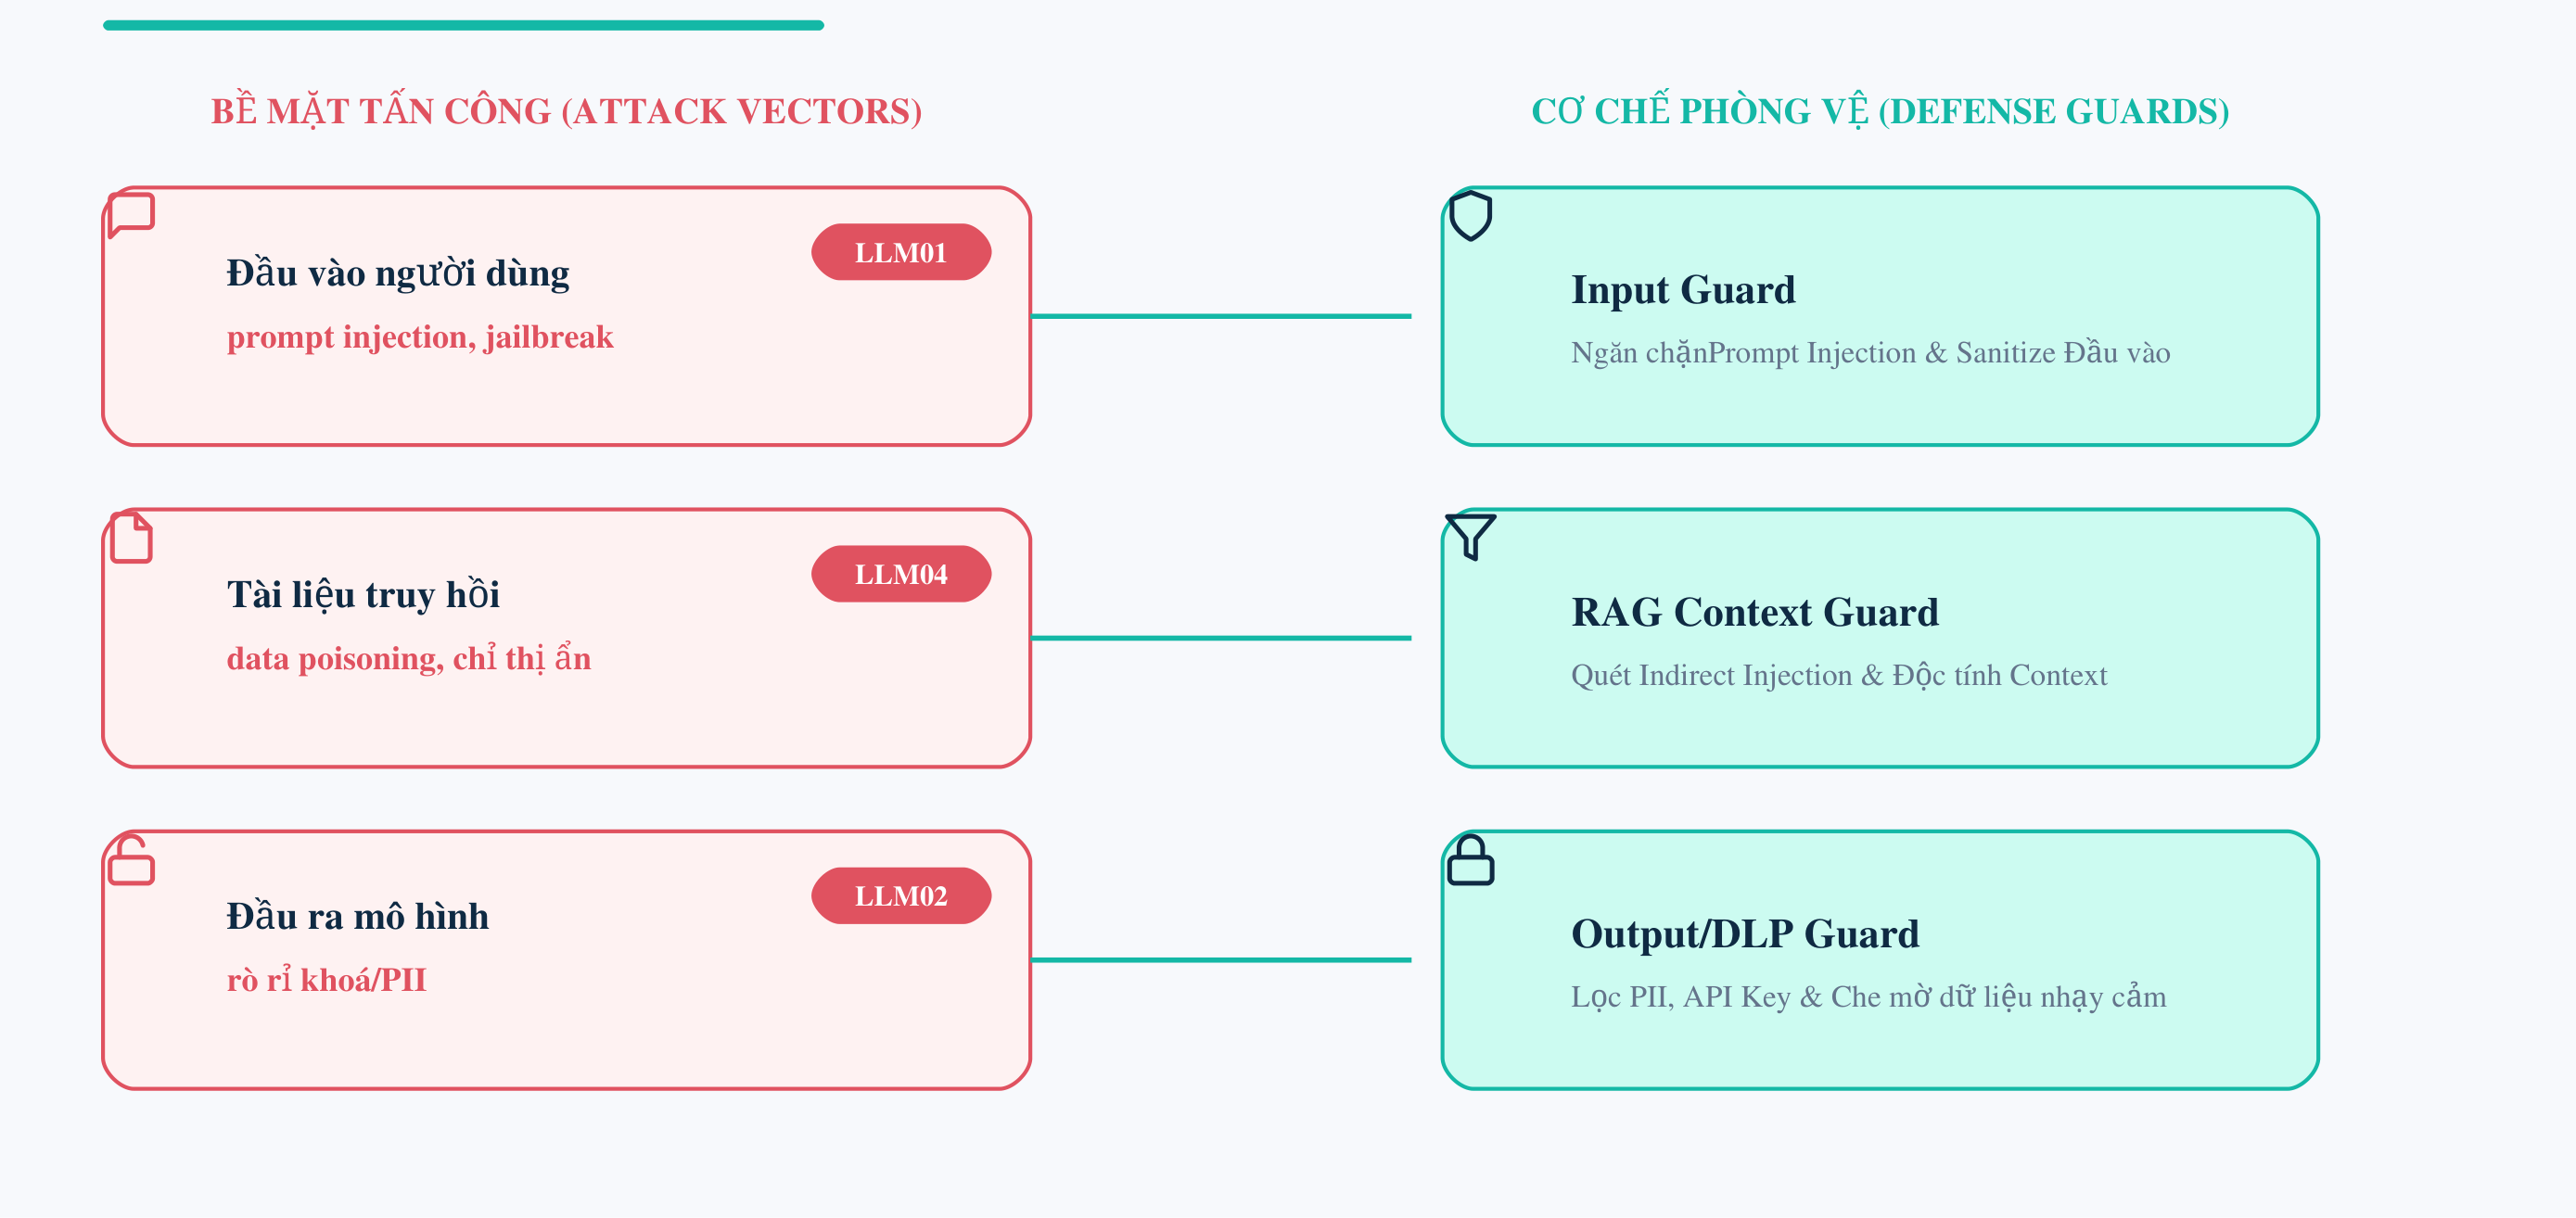
\includegraphics[width=0.75\linewidth]{figures/fig-threat-model.png}
\caption{Mô hình mối đe doạ: ba bề mặt tấn công và guard phòng vệ tương ứng}
\label{fig:threat-model}
\end{figure}

Hình~\ref{fig:threat-model} ánh xạ ba bề mặt tấn công của hệ thống RAG/LLM sang
lớp guard xử lý và mục tương ứng trong OWASP LLM Top 10: đầu vào người dùng
(prompt injection, jailbreak --- LLM01) do Input Guard xử lý; tài liệu truy hồi
(data poisoning, chỉ thị ẩn --- LLM04) do RAG Context Guard xử lý; và đầu ra mô
hình (rò rỉ khoá, PII --- LLM02) do Output/DLP Guard xử lý.

\section{Kết luận chương}

Chương này xác lập nền tảng: LLM/RAG mang lại năng lực mới nhưng mở rộng bề mặt tấn công. Kiểm soát cần đa lớp (đầu vào, ngữ cảnh, đầu ra) và phải đo được bằng kiểm thử có kiểm soát. Chương tiếp theo chuyển sang phân tích yêu cầu và thiết kế hệ thống của đề tài.
